%%%%%%%%%%%%%%%%%%%%%%%%%%%%%%%%%%%%%%%%%%%%%%%%%%%%%%%%%%%%%%%%%%%%%%%%%%%%%%%
% i7 Seminar Report Template
% Version June 23, 2023

\documentclass[a4paper,11pt,DIV=15]{scrartcl} % Do not edit this line.


%%%%%%%%%%%%%%%%%%%%%%%%%%%%%%%%%%%%%%%%%%%%%%%%%%%%%%%%%%%%%%%%%%%%%%%%%%%%%%%
% Preamble

% Page Geometry, Typography and Encoding
\usepackage[utf8]{inputenc}
\usepackage[T1]{fontenc}
\usepackage{microtype}
\renewcommand{\phi}{\varphi}
\renewcommand{\epsilon}{\varepsilon}
% \renewcommand{theta}{\vartheta} % if you want

% Math packages
\usepackage{amsmath}
\usepackage{amssymb}
\usepackage{amsthm}
\usepackage{mathtools}

% Floats
\usepackage{float}
\usepackage{booktabs}
\usepackage{tikz}
\usetikzlibrary{positioning,arrows.meta}

% Colors
\usepackage{xcolor} %already loaded by tikz, but here for completeness
% RWTH colors
% blue violet purple carmine red magenta orange yellow grass cyan gold silver
\definecolor{rwth-blue}{cmyk}{1,.5,0,0}\colorlet{rwth-lblue}{rwth-blue!50}\colorlet{rwth-llblue}{rwth-blue!25}
\definecolor{rwth-violet}{cmyk}{.6,.6,0,0}\colorlet{rwth-lviolet}{rwth-violet!50}\colorlet{rwth-llviolet}{rwth-violet!25}
\definecolor{rwth-purple}{cmyk}{.7,1,.35,.15}\colorlet{rwth-lpurple}{rwth-purple!50}\colorlet{rwth-llpurple}{rwth-purple!25}
\definecolor{rwth-carmine}{cmyk}{.25,1,.7,.2}\colorlet{rwth-lcarmine}{rwth-carmine!50}\colorlet{rwth-llcarmine}{rwth-carmine!25}
\definecolor{rwth-red}{cmyk}{.15,1,1,0}\colorlet{rwth-lred}{rwth-red!50}\colorlet{rwth-llred}{rwth-red!25}
\definecolor{rwth-magenta}{cmyk}{0,1,.25,0}\colorlet{rwth-lmagenta}{rwth-magenta!50}\colorlet{rwth-llmagenta}{rwth-magenta!25}
\definecolor{rwth-orange}{cmyk}{0,.4,1,0}\colorlet{rwth-lorange}{rwth-orange!50}\colorlet{rwth-llorange}{rwth-orange!25}
\definecolor{rwth-yellow}{cmyk}{0,0,1,0}\colorlet{rwth-lyellow}{rwth-yellow!50}\colorlet{rwth-llyellow}{rwth-yellow!25}
\definecolor{rwth-grass}{cmyk}{.35,0,1,0}\colorlet{rwth-lgrass}{rwth-grass!50}\colorlet{rwth-llgrass}{rwth-grass!25}
\definecolor{rwth-green}{cmyk}{.7,0,1,0}\colorlet{rwth-lgreen}{rwth-green!50}\colorlet{rwth-llgreen}{rwth-green!25}
\definecolor{rwth-cyan}{cmyk}{1,0,.4,0}\colorlet{rwth-lcyan}{rwth-cyan!50}\colorlet{rwth-llcyan}{rwth-cyan!25}
\definecolor{rwth-teal}{cmyk}{1,.3,.5,.3}\colorlet{rwth-lteal}{rwth-teal!50}\colorlet{rwth-llteal}{rwth-teal!25}
\definecolor{rwth-gold}{cmyk}{.35,.46,.7,.35}
\definecolor{rwth-silver}{cmyk}{.39,.31,.32,.14}

% Hyperlinks and Cross-References
\usepackage{hyperref}
\usepackage[capitalise,noabbrev]{cleveref}
\hypersetup{%
	pdftoolbar=false,
	pdfmenubar=false,
	colorlinks,
	%pdfborderstyle={/S/U/W 1.25},
	urlcolor={rwth-magenta},
	linkcolor={rwth-red},
	citecolor={rwth-green}
}

\theoremstyle{plain}
\newtheorem{theorem}{Theorem}
\newtheorem{proposition}[theorem]{Proposition}
\newtheorem{lemma}[theorem]{Lemma}
\newtheorem{corollary}[theorem]{Corollary}
\newtheorem{conjecture}[theorem]{Conjecture}
\newtheorem{claim}[theorem]{Claim}
\theoremstyle{definition}
\newtheorem{definition}[theorem]{Definition}
\newtheorem{remark}[theorem]{Remark}



% Misc packages
\usepackage{lipsum}



%%%%%%%%%%%%%%%%%%%%%%%%%%%%%%%%%%%%%%%%%%%%%%%%%%%%%%%%%%%%%%%%%%%%%%%%%%%%%%%
% Document


\begin{document}

%TODO Insert topic of seminar, e.g. Theoretical Topics in Data Science or Complexity Theory
\subtitle{Seminar ``[Topic of Seminar]''}
\date{\today}
\publishers{RWTH Aachen University}	% Do not edit this line.

%TODO Change this to your report title.
\title{[Title of Your Seminar Report]}

%TODO Change this to your name.
\author{[Your name]}

\maketitle


%TODO Provide a short abstract for your report.
\begin{abstract}
	\lipsum[1-2]
\end{abstract}

\thispagestyle{empty}

\clearpage

%TODO The content of your report goes below.

\section{General Information}
Your report should be written using this template and be of \textbf{6 
pages, excluding title page and bibliography}. Replace the title and the author 
command above with the title of your report and your name. Please 
\textbf{rename your file}, so that it includes your last name and (a fragment
of) the title of your report.

Please note the following general guidelines.
\begin{itemize}
	\item \textbf{Do} use sections to structure your report.
	\item \textbf{Do} use \verb|amsthm| blocks for definitions, theorems and so
		on (see \cref{s:math}).
	\item \textbf{Do} emphasize important notions with \verb|\emph{...}| on 
		their first appearrance.
	\item \textbf{Do not} use a table of contents (\verb|\tableofcontents|).
	\item \textbf{Do not} tamper with the page geometry or the font size to stay
		within the page limit. Also do not use unnecessary vertical spacing 
		commands for this purpose.
\end{itemize}

All packages loaded by the template are part of \TeX{} Live.





%%%%%%%%%%%%%%%%%%%%%%%%%%%%%%%%%%%%%%%%%%%%%%%%%%%%%%%%%%%%%%%%%%%%%%%%%%%%%%%
\section{Math}\label{s:math}
Enclose text in math using \verb|\text{...}|. Make sure that the horizontal
space to the surrounding math is right:
\begin{itemize}
	\item \verb|$\{ x \in \mathbb{N} \colon x \text{is even}\}$| yields
		$\{ x \in \mathbb{N} \colon x \text{is even}\}$.
	\item \verb|$\{ x \in \mathbb{N} \colon x \text{ is even}\}$| yields
		$\{ x \in \mathbb{N} \colon x \text{ is even}\}$.
\end{itemize}
Function and operator names that are words or abbreviations (such as $\max$ and
$\log$) should be written with \verb|\operatorname{foo}|:
\begin{itemize}
	\item \verb|$foo(x)$| yields $foo(x)$.
	\item \verb|$\operatorname{foo}(x)$| yields 
		$\operatorname{foo}(x)$.
\end{itemize}
You can define operators with
\verb|\DeclareMathOperator{\foo}{foo}| from the \verb|mathtools|
package for easy reusability. This defines a math mode command
\verb|\foo| that is typeset like an operator name. Note that common
operator names such as $\log$, $\sin$, $\cos$, $\exp$, $\min$ and $\max$ are
predefined as \verb|\log|, \verb|\sin| and so on.\par

Sentences also end with a period if they end in a math environment. For inline
math, the period goes outside as in \verb|$f(x) = 2x+1$.|, for displaymath, the 
period stays inside as in \verb|\[f(x) = 2x+1.\]|. The \verb|cases| environment
also need correct punctuation:
\[
	D \colon \mathbb{R} \to \{0, 1\} \colon x \mapsto
	\begin{cases}
		1	& \text{if }x \in \mathbb{Q}\text,\\
		0	& \text{otherwise.}
	\end{cases}
\]

Important definitions should be put in a definition block like this.
\begin{verbatim}
	\begin{definition}
		A function $f \colon A \to B$ is called \emph{injective} if $x \neq y$
		implies $f(x) \neq f(y)$.
	\end{definition}
\end{verbatim}
This renders as follows.
\begin{definition}
	A function $f \colon A \to B$ is called \emph{injective} if $x \neq y$
	implies $f(x) \neq f(y)$.
\end{definition}
Similar environments are \verb|theorem|, \verb|lemma| and \verb|corollary|.
\begin{theorem}
	If $A$ and $B$ are sets and $f \colon A \to B$ an injective function, then
	$\lvert A \rvert \leq \lvert B \rvert$.
\end{theorem}

You can give a special name to these blocks by putting it in square brackets. 
For example, \verb|\begin{theorem}[K\H{o}nigs Lemma]| results in the following.

\begin{theorem}[K\H{o}nigs Lemma]
	\label{thm:konigs-lemma}
	Every infinite, finite-branching tree contains an infinite path.
\end{theorem}

Put the proofs in \verb|proof| environments:
\begin{verbatim}
	\begin{proof}
		Left as an exercise to the reader.
	\end{proof}
\end{verbatim}

This renders as follows.
\begin{proof}
	Left as an exercise to the reader.
\end{proof}

%%%%%%%%%%%%%%%%%%%%%%%%%%%%%%%%%%%%%%%%%%%%%%%%%%%%%%%%%%%%%%%%%%%%%%%%%%%%%%%
\section{Color}
The template has the \verb|xcolor| package loaded and additionally defines the
color scheme of RWTH Aachen University. The documentation of \verb|xcolor|,
including the list of color names can be found on
\href{https://ctan.org/pkg/xcolor}{CTAN}, The naming convention for RWTH colors
is \verb|rwth-blue,rwth-orange,...| and for lighter variants \verb|rwth-lblue|
and \verb|rwth-llblue| and similar for the other colors.





%%%%%%%%%%%%%%%%%%%%%%%%%%%%%%%%%%%%%%%%%%%%%%%%%%%%%%%%%%%%%%%%%%%%%%%%%%%%%%%
\section{Figures and Tables}
Figures can be created using Ti\textit{k}Z. You can find examples on 
\href{https://www.texample.net/tikz}{\TeX{}ample.net}.\par
\begin{figure}[H]
	\begin{center}
	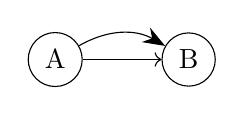
\begin{tikzpicture}[every node/.style={draw,circle}]
		\node (A) at (0,0) {A};
		\node[right=of A] (B) {B};
		% \node (B) at (2,0) {B};
		\draw[->] (A) to (B);
		\draw[out=30,in=150,-{Stealth[length=0.8em]}] (A) to (B);
	\end{tikzpicture}
	\end{center}

\end{figure}

It is preferred that you abstain from using including raster graphics in your
report, like scans of drawings or images copied from your sources. 
Vector graphics created outside of \LaTeX are also accepted (but try to use 
similar fonts and fontsizes in there). 

You can create nice looking tables with the included \verb|booktabs|-package:

\begin{figure}[H]
	\centering
	\begin{tabular}{ c l l }
		\toprule
		\textbf{Symbol}	& \textbf{Name}				& \textbf{Value}\\
		\midrule
		$\pi$ 				& (Archimedes' constant)	& $3.1415926535\dots$\\
		$e$					& Euler's number				& $2.7182818284\dots$\\
		$\Phi$				& Golden ratio					& $1.6180339887\dots$\\
		\bottomrule
	\end{tabular}
	\caption{An example table.}
\end{figure}





%%%%%%%%%%%%%%%%%%%%%%%%%%%%%%%%%%%%%%%%%%%%%%%%%%%%%%%%%%%%%%%%%%%%%%%%%%%%%%%
\section{Typographic Recommendations}
\begin{itemize}
	\item Use \verb|$\ell$| (rendering as $\ell$) instead of \verb|$l$| 
		(rendering as $l$).
	\item This template uses \verb|\varphi| and \verb|\varepsilon| for $\phi$
		and $\epsilon$ instead of the default symbols as they look nicer.
		You may also redefine $\theta$ to \verb|\vartheta| ($\vartheta$).
	\item Instead of $\times$ (\verb|\times|) or $*$ (\verb|*|), use $\cdot$
		(\verb|\cdot|) for multiplication.
\end{itemize}
You can find useful information on English usage and on typography for your 
paper in \cite{Higham1998}. You can find common phrases in \cite{Trzeciak2005}.





%%%%%%%%%%%%%%%%%%%%%%%%%%%%%%%%%%%%%%%%%%%%%%%%%%%%%%%%%%%%%%%%%%%%%%%%%%%%%%%
\section{Cross-References and Citations}\label{sec:ref}
Sources should be cited using \textsc{Bib}\TeX{}. \textsc{Bib}\TeX{}
automatically lists the cited sources at the end of the document. Note that
you need to compile the document as follows when using \textsc{Bib}\TeX{}:
\begin{center}
	pdflatex $\to$ bibtex $\to$ pdflatex $\to$ pdflatex.
\end{center}
Make sure that author names are spelled properly with all diacritcs, cf.\@ \cref{thm:konigs-lemma}. 
If possible, include digital object identifiers (DOIs) in your \textsc{Bib}\TeX{} entries.
The \href{https://dblp.uni-trier.de/}{dblp computer science bibliography}
is a good source for \textsc{Bib}\TeX{} entries.

For references within the report, you can set jump marks using 
\verb|\label{foo}|. They can be references with \verb|\ref{foo}|. This template
loads the \verb|cleveref| package, so you can also reference with 
\verb|\cref{foo}|:
\begin{itemize}
	\item \verb|Section~\ref{sec:ref}| yields: Section~\ref{sec:ref}.
	\item \verb|\cref{sec:ref}| yields: \cref{sec:ref}.
\end{itemize}


\section{Numbering and Referencing Equations}

Equations inserted via \verb|\[ ... \]| are not numbered:
\[
\sum_{i=1}^n i = \frac{n(n+1)}{2}
\]
If you want to refer to equations anywhere else in your report, use for example
the \verb|equation| environment and labels (\verb|\label{eq:geometric}|), cf.\@ \cref{sec:ref}.
This yields a numbered equation and allows references pointing to it:
\begin{equation} \label{eq:geometric}
\sum_{i=0}^n q^i = \frac{1 - q^{n+1}}{1-q} 
\end{equation}
You can then refer to your equation using \verb|\cref{eq:geometric}|: \cref{eq:geometric}.

When writing several equations, for example for a longer computation, the \verb|align|
environment is often useful. By default, all lines in an \verb|align| environment are
numbered. It is unlikely that you need to refer to all lines of such a computation later.
Here the \verb|\nonumber| command comes in handy. It inhibits the number of the line it is
place in. If you do not any of the equations numbered, use the \verb|align*| environment
instead.
\begin{align}
\int x \sin x dx 
&= - x \cos x + \int \cos x dx \nonumber \\
&= - x \cos x + \sin x.
\end{align}


\clearpage

\bibliographystyle{plainurl}
\bibliography{references.bib}





\end{document}





